\subsection{Stability study}
    For practical reasons it is important to not only evaluate the models on high-quality data exclusively, but also to know how the predictions will degrade when the input's data quality decreases. Having a model for fluorescence \textit{in silico} labeling that can additionally alarm end use when the predictions should not be relied upon is very useful in practice. Although the DIC microscopy is a relatively easy technique, there are still setting up procedures taking place that can be prone to errors. Additionally, as the models are not easily generalizable across phenotypes as well as between fixed and not fixed cells, an alarming system that is able to catch these situations would be useful to save time and cost of lab work. In order to measure the stability or robustness of the models towards data degeneration they were evaluated on the corrupted or "bad" input DIC images. There are two sources of "bad" images that can be used for such estimations. The first are actually corrupted images made in the laboratory. Such corruptions may come from different sources: for example, an oil bubble landed on the microscope lenses, low density of the cell on the image, over- or underexposure during image acquisition. Another source of image corruption would be images with artificial or pseudocorruptions created manually via image processing. 
    
    %This chapter first provides a description of artificial corruptions used to evaluate previously trained models on. Afterwards the real examples of corruptions acquired from the lab are 
    \subsubsection{Artificial corruptions}
        
In this subsection results from evaluating models on three types of artificial image corruption are presented, namely: defocus blur that imitates the defocus of the microscope lenses, changes in brightness and changes in contrast. Every corruption  has different effects on the prediction of the model based on its severity level. Therefore it is important to evaluate the error-rate (in this case a loss function) for the predictions for different severity levels of each corruption type presented. It is also important to perform a visual evaluation of the model's predictions on corrupted data. Each corruption $c$ has severity levels $s$, where $-5 \leq s \leq 5$ ($0 \leq s \leq 5$ for defocus blur corruption). $0$ here corresponds to an original image without corruption. It is important to keep in mind that although severity levels were chosen to be as much comparable between one another as possible, they still might have differences in their strengths. For example, contrast has much stronger effect on predictions than brightness changes. Three types of artificial image corruption are presented below.

\subsubsection{Defocus Blur}
\label{section:defocus-blur}
Defocus blur corruption imitates the effect of defocus on the microscope. The blur is applied to the image by convolving it with a special defocus kernel. There are two tunable parameters for this corruption type: the first one is the radius of the circle in the kernel $r$, and the second one is the blur strength parameter $s$. An example of the kernel with radius $r$ is shown in the Figure \ref{fig:defocus-blur-kernel}. This kernel is then simply applied to an image via $cv2.filter2D$ function.

\begin{figure}[htb]
	\begin{center}
		
\includegraphics[width=0.2\linewidth]{bilder/stability/defocus-blur-kernel.png}
		\caption{Defocus blur kernel}\label{fig:defocus-blur-kernel}
	\end{center}
\end{figure}

\subsubsection{Brightness}
Different brightness levels are also an important image corruption to perform tests on. Brightness variations appear often in the dataset during image acquisition. In order to change the brightness, an image from the RGB format was translated into HSV format, which stands for hue, saturation and value. This is also one of the popular formats to represent an image. To make an image brighter or darker, one can simply add or subtract a parameter $s$ in a value channel for each pixel $x_{i,j}$ correspondingly. This parameter is often called bias. The bigger absolute value of this of this change, the stronger a corruption will occur.

\begin{equation}
    \hat{x}_{i, j} = x_{i, j} + s
\end{equation}

\subsubsection{Contrast}
In contrast to adding a constant value pixelwise to an image in order to change a contrast level, one can perform a multiplication of an image with another constant $s$. This parameter is often called gain.

\begin{equation}
    \hat{x}_{i, j} = s * x_{i, j}
\end{equation}

For both contrast and brightness changes one can use $cv2.convertScaleAbs()$ from the OpenCV library. This method directly accepts gain and bias parameters and clips the image to stay within the allowed range of values.

The values of hyperparameters used in corruptions (kernel radius, gain and bias) are stretched across the range of severity levels and presented in Table \ref{table:corruption-hyperparameters}.
\begin{table}[htb]
    \centering
    \caption{Hyperparameterization for different artificial corruption severities}
        \begin{adjustbox}{width=1\textwidth}
            \begin{tabular}{|l||*{11}{c|}}\hline
                \backslashbox{Corruption}{Severity}
                &\makebox[3em]{-5}
                &\makebox[3em]{-4}
                &\makebox[3em]{-3}
                &\makebox[3em]{-2}
                &\makebox[3em]{-1}
                &\makebox[3em]{0}
                &\makebox[3em]{1}
                &\makebox[3em]{2}
                &\makebox[3em]{3}
                &\makebox[3em]{4}
                &\makebox[3em]{5}
                \\\hline\hline
                Defocus blur (radius) &-&-&-&-&-&0&0.5&1.0&1.5&2&3\\\hline
                Contrast (gain) &3.5&3.0&2.5&2.0&1.5&1&0.9&0.8&0.7&0.5&0.3\\\hline
                Brightness (bias) &-150&-135&-120&-90&-50&0&50&90&120&135&150\\\hline
            \end{tabular}
        \end{adjustbox}
    \label{table:corruption-hyperparameters}
\end{table}

Severity level of $-5$ for contrast represents a highly contrastive image, while $5$ is a very low contrast image. For brightness corruption levels of $-5$ and $5$ correspond to images with very low and high brightness respectively. And defocus blur corruption has only 5 levels of severity, ranging from the original image (level $0$) to the image with a stronger blur (level $5$).
\begin{figure}[H]
	\begin{center}
		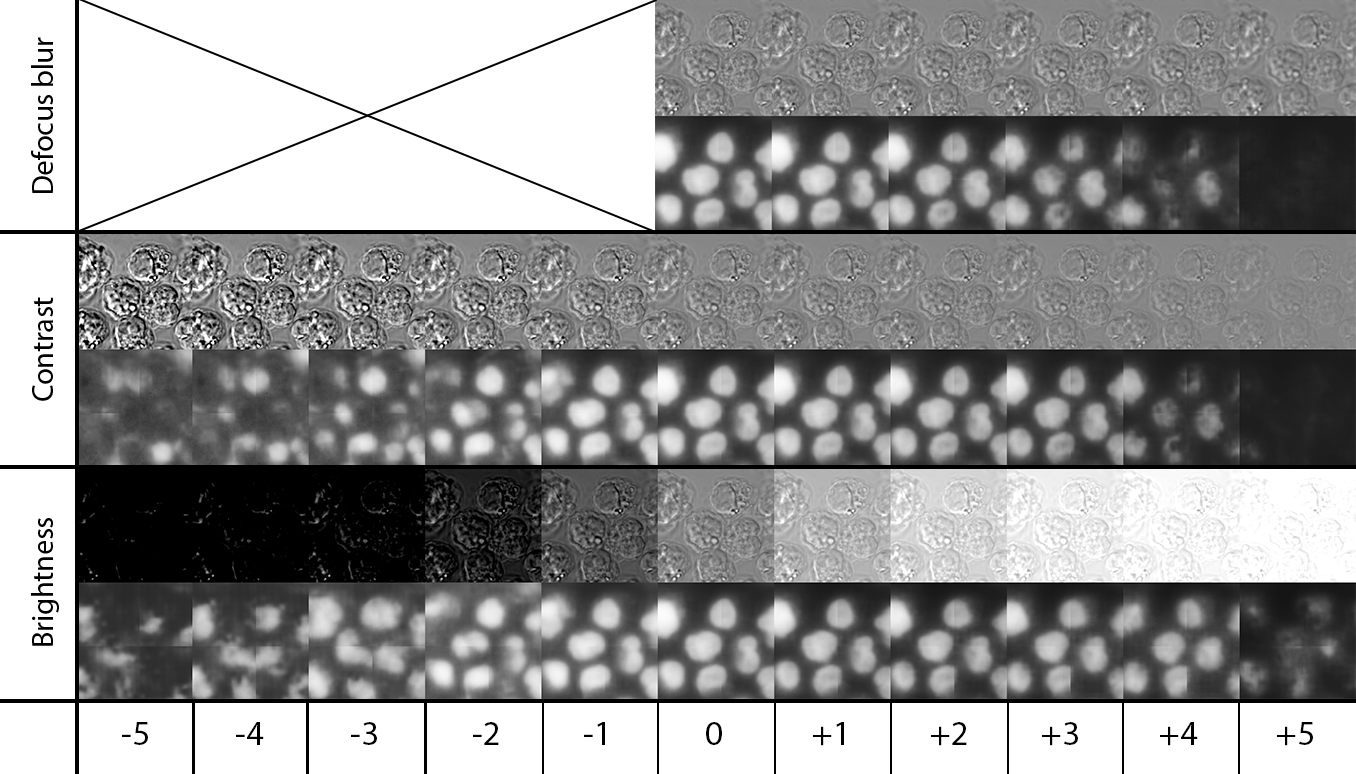
\includegraphics[width=0.5\linewidth]{bilder/corruptions.png}
		\caption{Influence of artificial corruptions on the predictions}
        \label{fig:artificial-corruptions}
	\end{center}
\end{figure}

One can observe the input image change for each of the corruptions along with the change of prediction of nuclei model in Figure \ref{fig:artificial-corruptions}. It can be clearly seen that the model's predictions are quite stable towards different brightness levels and contrast. However, the predictions on the crops are very sensible towards defocus blur corruption: DIC images with defocus blur levels $1-4$ are almost indistinguishable from the original image, yet the model's predictions degrade quite fast. This can be explained by the fact that the training dataset contains quite diverse data in terms of contrast and brightness levels and, as a result, the model is more stable towards these changes. Using defocus blur as an augmentation will help to solve this problem. This will be described in more detail in Section \ref{section:augments-againts-corruptions}.
\begin{figure}[htb]
	\begin{center}
		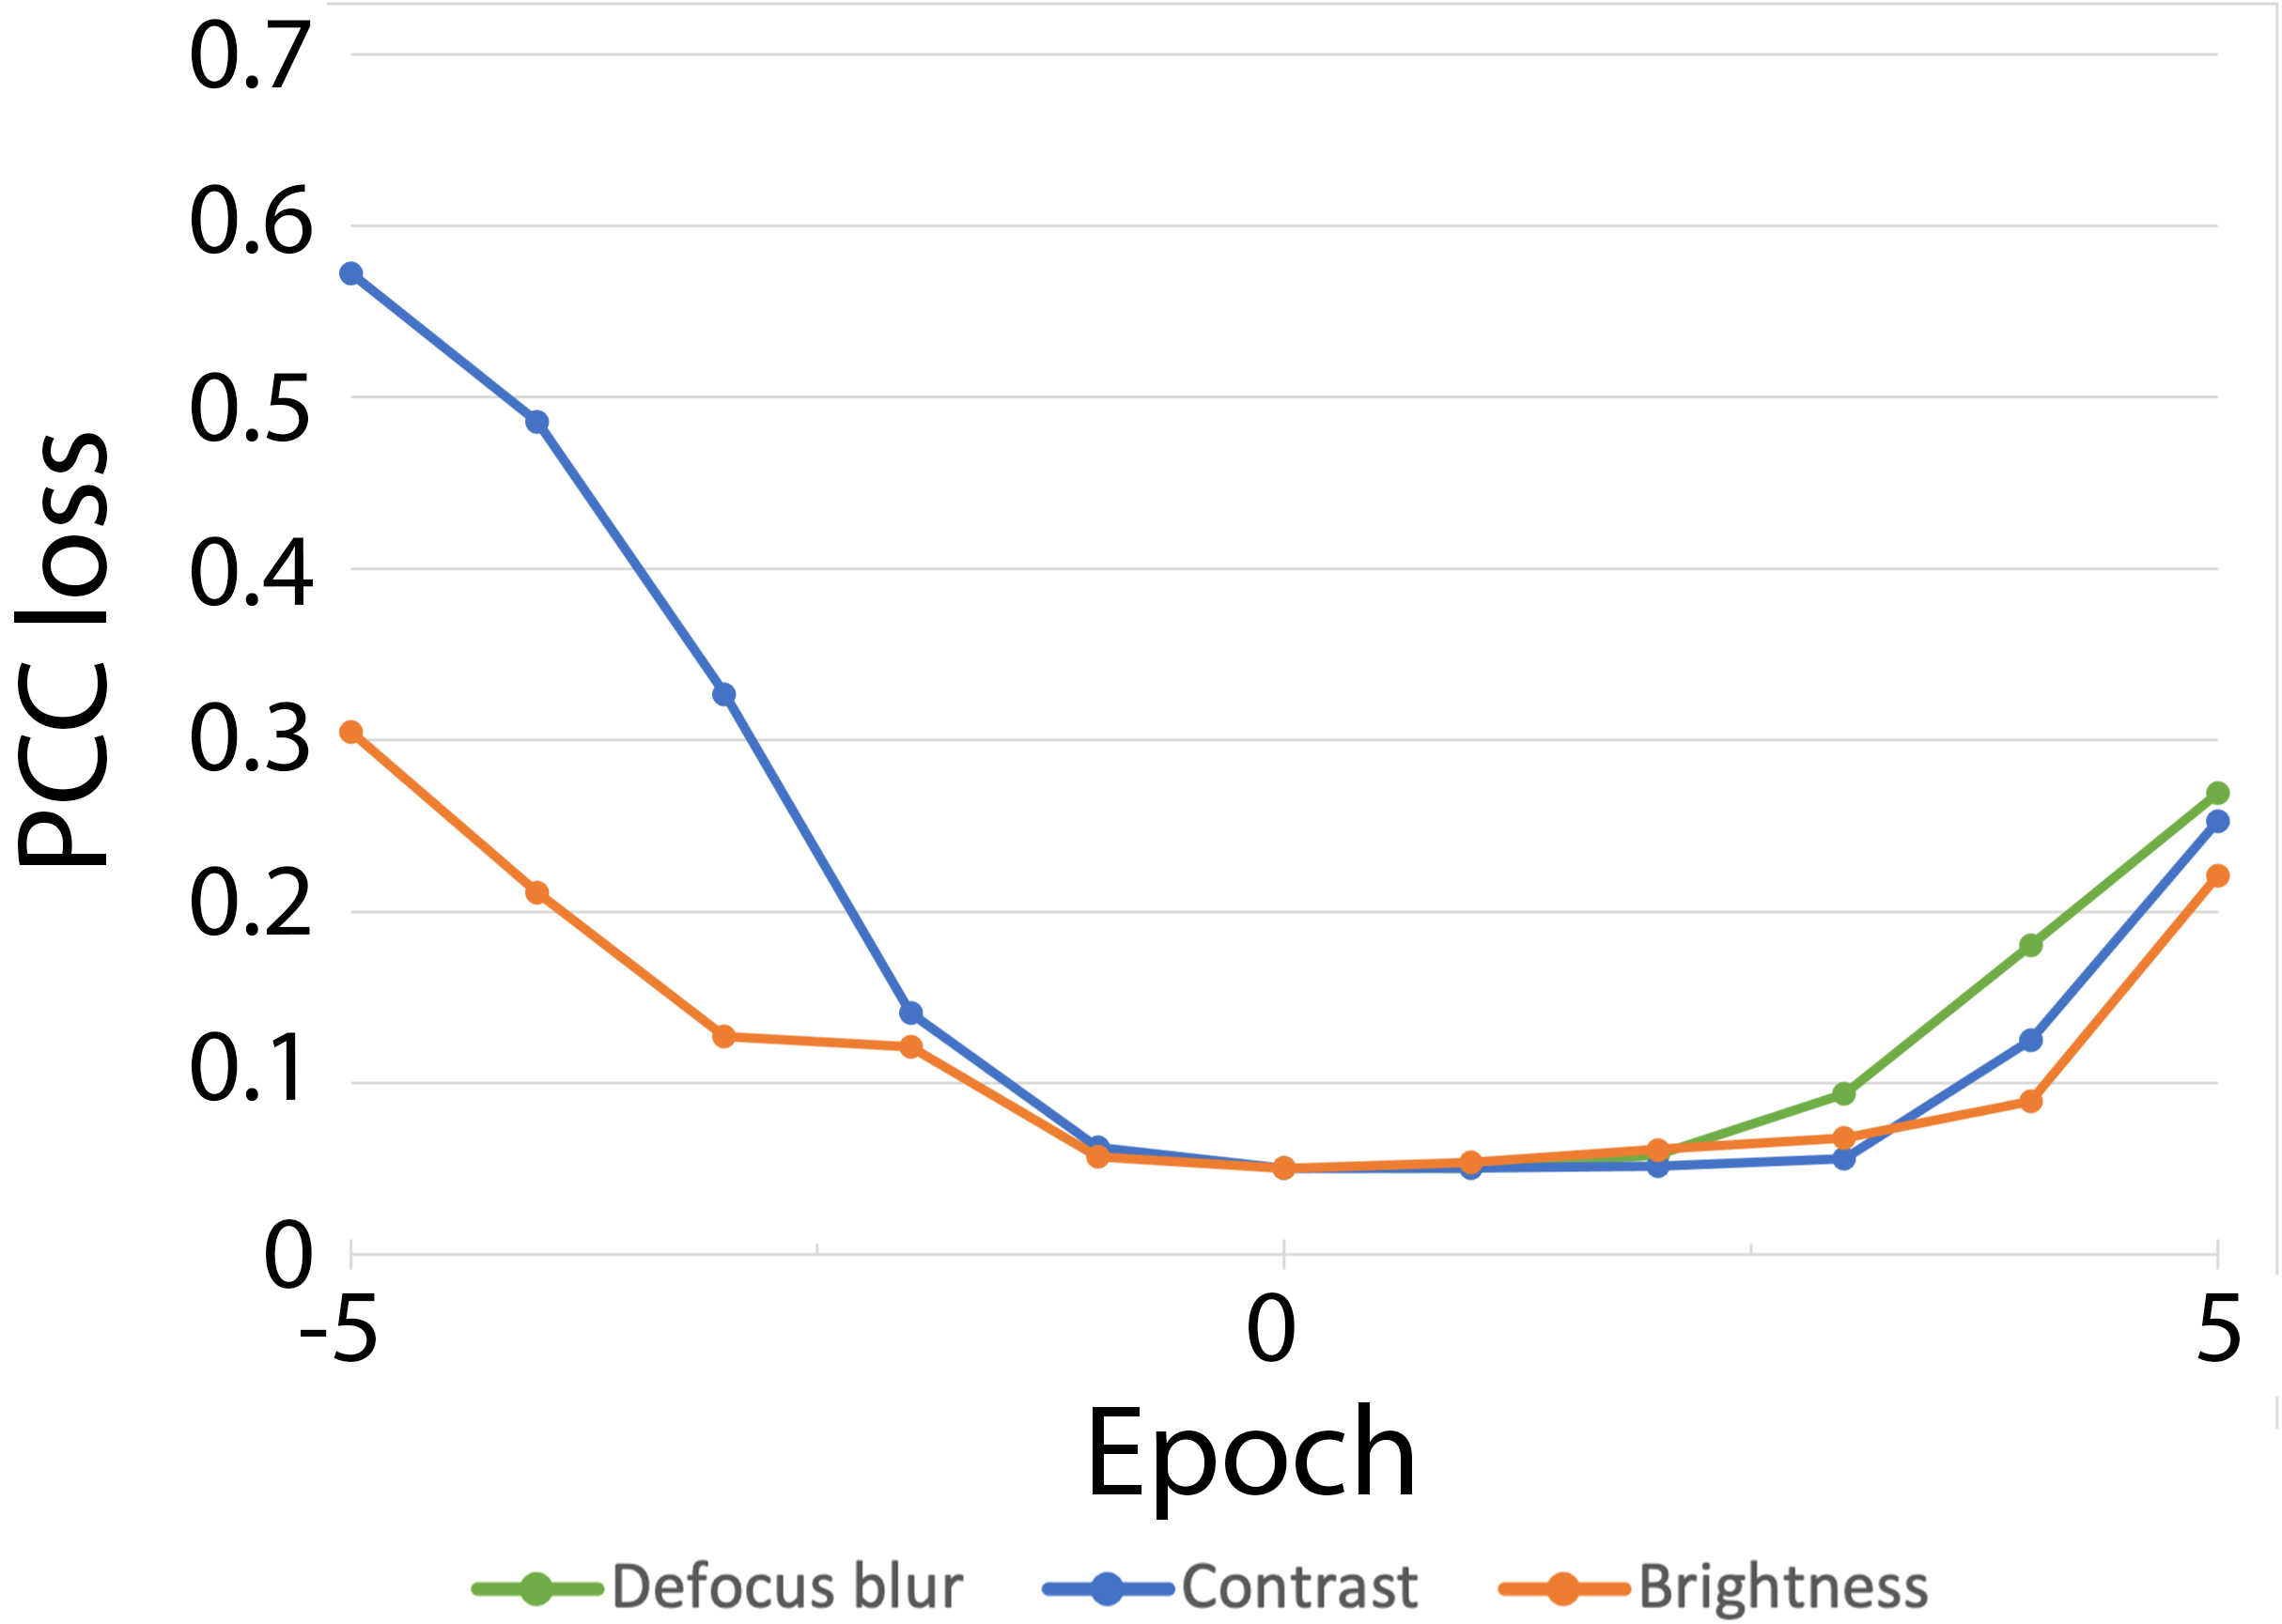
\includegraphics[width=0.5\linewidth]{bilder/corruptions-loss.png}
		\caption{Change of PCC loss for artificial corruptions}\label{fig:corruptions-loss}
	\end{center}
\end{figure}

Additionally, a change in PCC loss is presented in Figure \ref{fig:corruptions-loss}. This is a plot of PCC loss for different artificial corruptions. Loss increases for stronger severity levels. We can see that in a positive direction with defocus blur corruption the model degerates more quicker and that contrast corruptions change predictions more severely in the negative one.
    \subsubsection{Real corruptions}
        \label{section:real-corruptions}
        \paragraph{Not fixed cells imaging as corrupted input}
    \begin{figure}[H]
        \begin{center}
            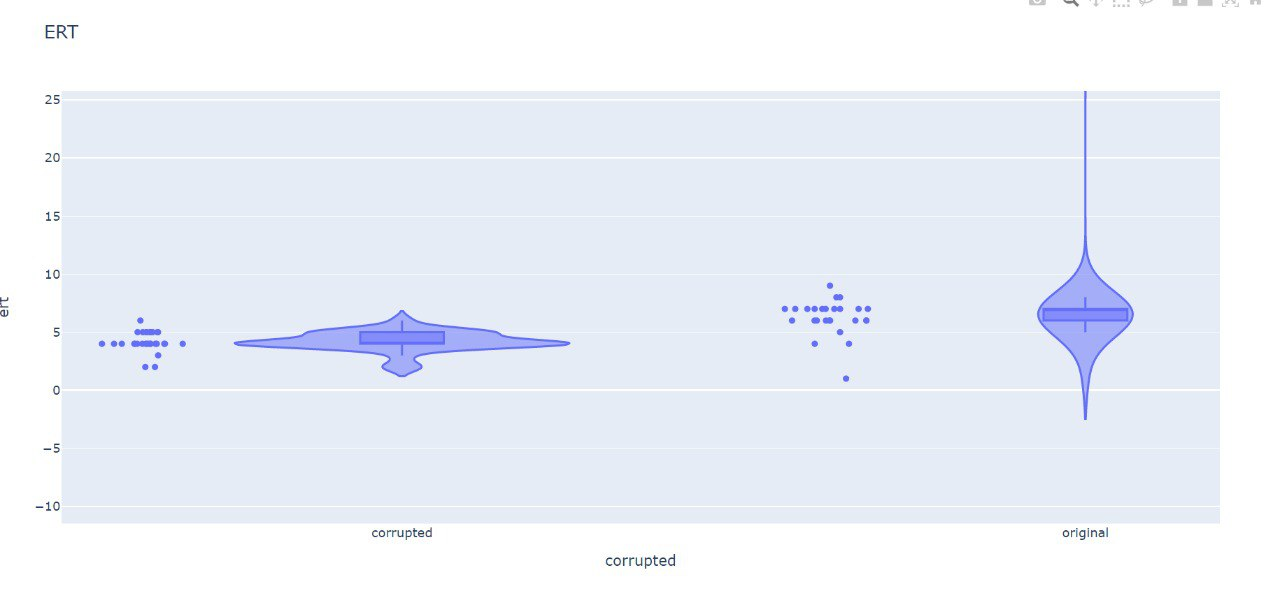
\includegraphics[width=0.5\linewidth]{bilder/drift-detection/online-fixed-vs-not-fixed.jpg}
            \caption{Online drift detection of not fixated cells}\label{fig:online-drift-not-fixed}
        \end{center}
    \end{figure}

    Scores of 0.91 however the threshold is 6, not corrupted data (fixed cells) mostly ert of 7 whereas corrupted data (not fixed cells) have an ert of 4. The threshold is therefore 6.

\paragraph{Real-world examples of corruptions}

    \subsubsection{Improving predictions with additional corruption augmentations}
        \label{section:augments-againts-corruptions}
        Going from observations of the models' stability towards different image brightness which is present in the datasets a new hypothesis was drawn. Introducing corruptions that we test on into the training should improve the predictions on corrupted data. Unfortunately, it is not possible to use real lab corruptions here as the data was provided only for testing on these difficult cases and was not stained. Without staining one cannot give a quantitative measure of the quality of the predictions. However, artificial corruptions can be applied here easily. Random changes in contrast, brightness and defocus blur of severity levels $-4$ and $4$ were added to the training augmentations. After the improved model was trained the predictions on the corrupted dataset became much better indeed (see Figure \ref{fig:augments-help}).

\begin{figure}[htb]
	\begin{center}
		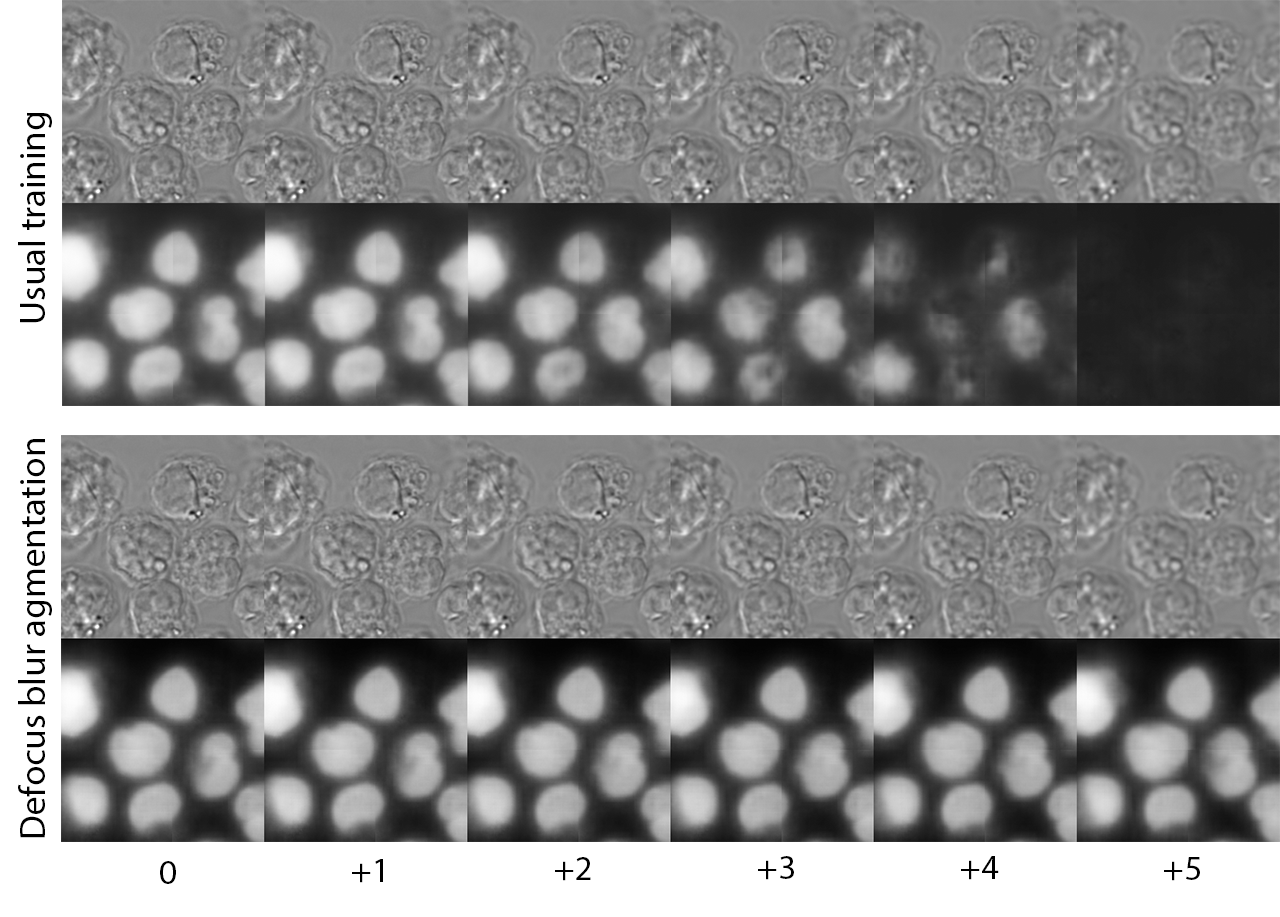
\includegraphics[width=0.4\linewidth]{bilder/stability/augments-help.png}
		\caption{Using corruptions as augmentations to improve predictions predictions}\label{fig:augments-help}
	\end{center}
\end{figure}

\subsubsection{Influence of corruptions on metrics for downstream tasks}
Additionally, since for artificial corruptions the ground truth data from staining is present, the difference in downstream metrics for models with and without augmentations was measured (see Table \ref{table:nuclei-corruptions-downstream-metrics-coefficients}), more specifically Spearman rank correlarion coefficients are compared. The calculation of downstream metrics remained the same except the thresholding algorithm was switched to a global one due to the time limit. This results in the wrong segmentation of some of the ground ground truth images. Therefore Spearman rank correlation coefficient is more repesentative here since it is more stable towards the outliers. The rest of the postprocessing procedure has remained the same apart from the application of artificial corruptions on the input data.

\begin{table}[htb]
    \centering
    \caption{Correlation coefficients for downstream tasks on nuclei}
        \begin{adjustbox}{width=0.7\linewidth}
            \begin{tabular}{|c|c|c|c|c|}\hline
                Contrast level&Number of nuclei&Total intensity&Mean intensity&Area\\\hline\hline
                +1&0.934&0.825&0.826&0.898\\\hline
                +2&0.932&0.820&0.819&0.899\\\hline
                +3&0.934&0.799&0.822&0.890\\\hline
                +4&0.804&0.439&0.671&0.540\\\hline
                +5&0.394&0.351&0.383&0.313\\\hline \hline
				Defocus blur level&Number of nuclei&Total intensity&Mean intensity&Area\\\hline\hline
                +1&0.934&0.832&0.827&0.905\\\hline
                +2&0.929&0.800&0.820&0.890\\\hline
                +3&0.934&0.756&0.8210&0.871\\\hline
                +4&0.838&0.361&0.666&0.501\\\hline
                +5&-0.072&-0.233&-0.231&0.07\\\hline
            \end{tabular}
        \label{table:nuclei-corruptions-downstream-metrics-coefficients}
        \end{adjustbox}
\end{table}

One can observe from the table above that the metrics degrade quite fast starting from the severity level $3$. The most affected metrics are the total and mean intensity. The number of organelles seems to be the most stable one until the very last severity level when the predictions turn almost completely black. 
    \subsubsection{Generalizability across phenotypes}
        TODO train the model on one phenotype and predict on the other, compare predictions (visually?)
        postprocessing with metrics then?